\documentclass[9pt]{beamer}
%----------------------------------------------------------
% Стиль презентации (выбрать понравившийся)
\usetheme{bmstu}
%------------------------------------------
% определения значений стандартных параметров
%----------------------------------------%
% общие определения
\newcommand{\UpperFullOrganisationName}{Министерство науки и высшего образования Российской Федерации}
\newcommand{\ShortOrganisationName}{МГТУ~им.~Н.Э.~Баумана}
\newcommand{\FullOrganisationName}{федеральное государственное бюджетное образовательное\newline учреждение высшего профессионального образования\newline <<Московский государственный технический университет имени Н.Э.~Баумана\newline (национальный исследовательский университет)>> (\ShortOrganisationName)}
\newcommand{\OrganisationAddress}{105005, Россия, Москва, ул.~2-ая Бауманская, д.~5, стр.~1}
%----------------------------------------%
\newcommand{\gitlabdomain}{sa2systems.ru:88}
%----------------------------------------------------------
\newcommand{\doctypesid}{kp} % vkr (выпускная квалификационная работа) / kp (курсовой проект) / kr (курсовая работа) / nirs (научно-исследовательская работа студента) / nkr (научно-квалификационная работа)

% Тема должна быть сформулирована так, чтобы рассказать, о чем работа, но сделать это так, чтобы у читателя возникло желание читать аннота-цию. При формулировке темы не следует стараться рассказать о работе всё. Пример корректной темы: "Математическое моделирование процесса размножения медуз в Южно-Китайском море". Пример некорректной темы: "Применение модели SIS для моделирования процесса размножения медуз в Южно-Китайском море с использованием метода Рунге-Кутты и многопроцессорных вычислительных систем".
\newcommand{\Title}{Разработка механизма вывода типов с использованием системы типов Хиндли-Милнера}%{}
\newcommand{\TitleSource}{кафедра} % кафедра, предприятие, НИР, НИР кафедры, заказ организации

\newcommand{\SubTitle}{по дисциплине <<Модели и методы анализа проектных решений>>} % Методы оптимизации
\newcommand{\faculty}{<<Робототехника и комплексная автоматизация>>}
\newcommand{\facultyShort}{РК}
\newcommand{\department}{<<Системы автоматизированного проектирования (РК-6)>>}
\newcommand{\departmentShort}{РК-6}

\newcommand{\Author}{Никитин В.Л.}
\newcommand{\AuthorFull}{Никитин Владимир Леонидович}
\newcommand{\ScientificAdviserPosition}{доктор физико-математических наук}    % Должность научного руководителя
\newcommand{\ScientificAdviser}{Соколов А.П.}    % Научный руководитель
\newcommand{\ConsultantA}{Соколов А.П.}                % Консультант 1
% \newcommand{\ConsultantB}{@Фамилия~И.О.@}				% Консультант 2
\newcommand{\Normocontroller}{Грошев~С.В.}        % Нормоконтролёр
\newcommand{\group}{РК6-75Б}
\newcommand{\Semestr}{осенний семестр} % Например: осенний семестр или весенний семестр
\newcommand{\BeginYear}{2023}
\newcommand{\Year}{2024}
\newcommand{\Country}{Россия}
\newcommand{\City}{Москва}
\newcommand{\TaskStatementDate}{<<\underline{\textit{01}}>> \underline{октября} \Year~г.} %Дата выдачи задания

\newcommand{\depHeadPosition}{Заведующий кафедрой}        % Должность руководителя подразделения
\newcommand{\depHeadName}{А.П.~Карпенко}        % Должность руководителя подразделения

% Цель выполнения 
\newcommand{\GoalOfResearch}{реализация системы вывода и проверки типов} % с маленькой буквы и без точки на конце

% Объектом исследования называют то, что исследуется в работе. Например, для указанной выше темы объектом может быть популяция медуз, но никак ни модель SIS, ни Южно-Китайское море, ни метод моделирования популяции медуз. 
\newcommand{\ObjectOfResearch}{система типов}

% Предмет исследований (уже чем объект, определяется, исходя из задач: формулируется как существительное, как правило, во множественном числе, определяющее "конкретный объект исследований" среди прочих в рамках более общего)
\newcommand{\SubjectOfResearch}{система типов Хиндли-Милнера}

% Основная задача, на решение которой направлена работа
\newcommand{\MainProblemOfResearch}{реализация алгоритма вывода типов на основе выбранной системы типов}

% Выполненные задачи
\newcommand{\SubtasksPerformed}{%
    В результате выполнения работы:
    \begin{inparaenum}[1)]
        \item спроектировано представление абстрактного синтаксического дерева в компиляторе;
        \item реализован семантический анализатор;
        \item показано, что компилятор успешно может вывести тип функции
    \end{inparaenum}}

% Ключевые слова (представляются для обеспечения потенциальной возможности индексации документа)
\newcommand{\keywordsru}{%
    теория типов, языки программирования, компиляторы, фукнциональное программирование, система типов Хиндли-Милнера} % 5-15 слов или выражений на русском языке, для разделения СЛЕДУЕТ ИСПОЛЬЗОВАТЬ ЗАПЯТЫЕ
\newcommand{\keywordsen}{%
    type theory, programming languages, compilers, functional programming, Hindley-Milner type system} % 5-15 слов или выражений на английском языке, для разделения СЛЕДУЕТ ИСПОЛЬЗОВАТЬ ЗАПЯТЫЕ

% Краткая аннотация
\newcommand{\Preface}{
	Работа посвящена реализации механизма вывода типов для языка программирования Kodept.
	Программирование выстроено вокруг глубокой математической теории.
	Благодаря этому появляются возможности для оптимизации, развития и улучшения языков посредством применения математики.
	Одним из важных применений является теория типов, которая помогает программисту в написании кода.
	В последнее время все больше и больше языков почерпывают что-то из этой области.
	Применение мощной системы типов позволяет зачастую снизить количество ошибок, возникающих при разработке.
} % с большой буквы с точкой в конце

%----------------------------------------%
% выходные данные по документу
\newcommand{\DocOutReference}{\Author. \Title\xspace\SubTitle. [Электронный ресурс] --- \City: \Year. --- \total{page} с. URL:~\url{https://\gitlabdomain} (система контроля версий кафедры РК6)}

%----------------------------------------------------------


%------------------------------------------
% определения значений стандартных общих параметров для различных документов, в т.ч. различных типов
%----------------------------------------------------------
% Информация о лицензии
\newcommand{\doclicense}{\copyright\xspace}
%\newcommand{\doclicense}{\includegraphics[width=0.1\textwidth]{../common_doc_spec/by.eps}\xspace}%\ccShareAlike
%----------------------------------------------------------
\newcommand{\doctextlicense}{\copyright\xspace} % Copyright ©
%\newcommand{\doctextlicense}{CC BY 4.0}% \ccAttribution
%----------------------------------------%
% общие определения
\newcommand{\UpperFullOrganisationName}{Министерство науки и высшего образования Российской Федерации}
\newcommand{\ShortOrganisationName}{МГТУ~им.~Н.Э.~Баумана}
\newcommand{\FullOrganisationName}{Московский государственный технический университет имени Н.Э.~Баумана}
\newcommand{\OrganisationAddress}{105005, Россия, Москва, ул.~2-ая Бауманская, д.~5, стр.~1}
%----------------------------------------%
\newcommand{\gitlabdomain}{gitlab.sa2systems.ru}
%----------------------------------------%
\newcommand{\faculty}{<<Робототехники и комплексной автоматизации>>}
\newcommand{\facultyShort}{РК}
\newcommand{\department}{<<Системы автоматизированного проектирования (РК-6)>>}
\newcommand{\departmentShort}{РК-6}
\newcommand{\departmentcloud}{\href{https://archrk6.bmstu.ru}{https://archrk6.bmstu.ru}}
%----------------------------------------------------------


%------------------------------------------
% общая кастомизируемая преамбула для презентаций
%----------------------------------------------------------
% Сохранение метаданных в PDF об авторе документа
\expandafter\hypersetup{%
		pdftitle={\Title},    	% title
		pdfauthor={\Author},    % author
		pdfcopyright={\doctextlicense, \begdate -- \Year, \Author. Все права защищены.},% -- \today,
		pdfsubject={\Title},   % subject of the document
%		pdfcreator={\pdftexbanner},   % creator of the document
		pdfpublisher={\department, \ShortOrganisationName},
		pdfcaptionwriter={\Author},
		pdfproducer={\Author, \begdate -- \Year, \ShortOrganisationName}, % producer of the document
		pdfkeywords={\keywordsru, \keywordsen}, % producer of the document
}
%----------------------------------------------------------
% final - удаляет все всплывающие комментарии
%\usepackage[author={\Author},opacity=0.1, final]{pdfcomment}
\usepackage[opacity=0.1]{pdfcomment}
%----------------------------------------------------------
\usepackage{tikz}
\usetikzlibrary{tikzmark}
\usetikzlibrary{matrix,automata,positioning,arrows,arrows.meta,graphs}
\usetikzlibrary{trees,topaths}
\usetikzlibrary{calc, circuits.ee.IEC}
\usetikzlibrary{patterns,decorations.pathmorphing,decorations.markings}
%----------------------------------------------------------

%------------------------------------------
% дополнительные параметры, имеющие отношение к данному документу
%----------------------------------------------------------
\newcommand\ddfrac[2]{\frac{\displaystyle #1}{\displaystyle #2}}
\newcommand\T{\textup{T}}
\def\argmin{\operatornamewithlimits{argmin}}
\def\argmax{\operatornamewithlimits{argmax}}
\def\diag{\operatornamewithlimits{diag}}
\def\dep{\operatornamewithlimits{dep}}
%----------------------------------------------------------
\newcommand{\bvec}[1]{\mbox{\mathversion{bold}${#1}$}}
\newcommand{\periodichnost}[1]{[\hspace{-2pt}[#1]\hspace{-2pt}]}
\newcommand{\volna}[1]{\mathop{#1}\limits\_{\sim}}
\newcommand{\crujok}[1]{#1}
\newcommand{\driv}[2]{\frac{d#1}{d#2}}
\newcommand{\pdriv}[2]{\frac{\partial #1}{\partial #2}}
\newcommand{\uparr}[1]{\overrightarrow{#1}}
\newcommand{\intThreeD}[1]{\hspace{6pt}\mathop{\int\hspace{-17pt}\int\hspace{-17pt}\int}\limits\_{#1}\hspace{6pt}}
\newcommand{\intTwoD}[1]{\hspace{6pt}\mathop{\int\hspace{-17pt}\int}\limits\_{\hspace{-6pt}#1}}
\newcommand{\mbf}[1]{\boldsymbol{#1}}
\renewcommand{\H}{\operatornamewithlimits{\mathit{H}}}
%----------------------------------------------------------
\newcommand{\multirowbox}[2]
{
   \parbox{#1}{\smallskip #2 \smallskip}
}
%----------------------------------------------------------

\declaretheorem[
  style=thrmstyle,
  title=Замечание,
  refname={замечание,замечания},
  Refname={Замечание,Замечания}
]{remark}

\theoremstyle{thrmstyle}

%\newtheorem{question}{Вопрос}
%\newtheorem{approval}{Утверждение}
%\newtheorem{demand}{Требование}
%\newtheorem{statement}{Утверждение}
%\newtheorem{syntax}{Синтаксис}
\let\definition\relax
\newtheorem{definition}{Определение}
%\newtheorem{designation}{Обозначение}
%\newtheorem{property}{Свойство}
\newtheorem{task}{Задача}
%\newtheorem{mathmod}{Математическая модель}
%\newtheorem{mytheorem}{Теорема}

%----------------------------------------------------------
\hyphenation{супер-ком-пью-тер-ный супер-ком-пью-тер-ное вы-со-ко-произ-во-ди-тель-ный}
%----------------------------------------------------------
\newcommand\MyProcess[3]
{
%\begin{tabular}{p{0.1\textwidth}p{0.9\textwidth}}
%&
\begin{lstlisting}[caption={#1}, label={#2}, language=ALGO, basicstyle=\small]
#3
\end{lstlisting}			
%\end{tabular}
}
%----------------------------------------------------------
\newcommand\myquote[2]{%
\textit{``#1''}
\begin{flushright}
\textcolor{gray}{#2}
\end{flushright}
}
%----------------------------------------------------------
\newcommand{\mydescr}[1]{%

\colorbox{black!5}{\parbox{0.7\textwidth}{\smaller[1]\textit{#1}}}
}
%----------------------------------------------------------
% вёрстка в две колонки
\newcommand\cols[4]
{\smaller[1]%
		\begin{columns}
		\begin{column}{#1}
    #2
		\end{column}
		\begin{column}{#3}
		#4
		\end{column}
		\end{columns}}
%----------------------------------------------------------
% вёрстка в две колонки двух блоков с itemize
\newcommand\colsblocks[4]
{\smaller[1]%
		\begin{columns}
		\begin{column}{0.5\textwidth}
		\begin{block}{#1}
		\begin{itemize}
			#2
		\end{itemize}
		\end{block}
		\end{column}
		\begin{column}{0.5\textwidth}
		\begin{block}{#3}
		\begin{itemize}
			#4
		\end{itemize}
		\end{block}
		\end{column}
		\end{columns}}
%----------------------------------------------------------
%\usepackage{ifthen}
%%----------------------------------------------------------
%\usepackage{totcount}
%%----------------------------------------------------------
%%\newboolean{shortversion}
%% #1 - current \doctype
%% #2 - destination document
%% #3 - text
%\newcommand{\myconditionaltext}[3]%
%{%
	%\ifthenelse{\equal{#1}{avtoreferat}\AND\equal{#2}{avtoreferat}}{#3}{}% short version
	%\ifthenelse{\equal{#1}{avtoreferat}\AND\equal{#2}{thesis}}{}{}% short version
	%\ifthenelse{\equal{#1}{avtoreferat}\AND\equal{#2}{presentation}}{}{}% short version
	%\ifthenelse{\equal{#1}{thesis}\AND\equal{#2}{presentation}}{}{}% short version
	%\ifthenelse{\equal{#1}{thesis}\AND\equal{#2}{thesis}}{#3}{}% short version
	%\ifthenelse{\equal{#1}{presentation}\AND\equal{#2}{presentation}}{#3}{}% short version
	%\ifthenelse{\equal{#1}{presentation}\AND\equal{#2}{thesis}}{\pdfcomment{#3}}{}% short version
%}

%----------------------------------------------------------
% #1 - Короткое название практики
% #2 - Короткое описание
% #3 - Назначение в форме itemize
% #4 - LaTeX код
\newcommand{\bestpractice}[4]{%
\subsection{#1}
\begin{frame}%[fragile]

{\smaller[1]
#2}

\begin{columns}[t]

\begin{column}{0.5\textwidth}
\begin{block}{Назначение}
{\smaller[1]%
#3}
\end{block}
\end{column}

\begin{column}{0.5\textwidth}
\begin{lstlisting}[language={TeX}, basicstyle=\scriptsize]
#4
\end{lstlisting}
\end{column}
\end{columns}

\end{frame}}
%----------------------------------------------------------
\newenvironment{arreqn}[2]
    {\smaller[1]
		\begin{block}{\smaller[1] #1}
    \begin{equation}\label{#2}
    \begin{array}{l}
    }
		{
    \end{array}
    \end{equation}
		\end{block}
    }
%----------------------------------------------------------





%------------------------------------------
% база терминов! 
%----------------------------------------------------------
%Термины и определения по тексту в большинстве случаев выделяются курсивом.

%%%%% для обычных newglossaryentry по умолчанию category==general.
%%%%% для обычных newabbreviation по умолчанию category==abbreviation.
%%%%% команда для создания своей категории \glscategory{<label>}

%\newabbreviation[category=initialism]{aINI}{aINI}{Расширенный формат \href{https://en.wikipedia.org/wiki/INI_file}{INI} (\href{http://sa2systems.ru/svn/public/sa2pdf/comfrm_ugd_AdvancedINI.pdf}{описание в документе <<Соколов А.П., Першин А.Ю. Руководство системного программиста. Формат данных Advanced INI (aINI) // Каркас системы comfrm – 2007-2017 – 18 стр.>>})}

%\newglossaryentry{AI}{name={ActionItem}, description={Функциональная возможность в системе \gls{dcs-gcd}. Понятие, введенное с целью определить абстракции над функциями различных типов, на основе которых возможно расширение функциональных возможностей разрабатываемой программной системы.}}

%\newglossaryentry{slver}{name={Solver}, description={Решатель системы \gls{dcs-gcd}. Регистрируется в таблице \textbf{com.slvrs} БД \gls{gcddb} \gls{dcs-gcd}.}}

\newabbreviation[category=initialism]{PO}{ПО}{Программное обеспечение}
\newabbreviation[category=initialism]{cm}{КМ}{Композиционный материал}
%\newabbreviation[category=initialism]{ASUTP}{АСУ ТП}{Автоматизированная система управления технологическими процессами.}
%\newabbreviation[category=initialism]{chb}{БзЧ}{базовая часть}

%\newglossaryentry{Gij}{name={$G_{ij}$},
	%	symbol={\ensuremath{\mathcal{\nu}}},
%	category=symbol,
%	description={модули сдвига ортотропного материала}}

%\GlsXtrEnableEntryCounting
%{abbreviation}% list of categories to use entry counting
%{2}% trigger value

%\GlsXtrEnableEntryCounting
%{symbol}% list of categories to use entry counting
%{2}% trigger value


%----------------------------------------------------------




%---------------------------------------------
\includeonly{%
,cpxsln_prs_prj_YYYY_Group_SurnameNS_intro
,cpxsln_prs_prj_YYYY_Group_SurnameNS_taskstatement
,cpxsln_prs_prj_YYYY_Group_SurnameNS_method
,cpxsln_prs_prj_YYYY_Group_SurnameNS_software
,cpxsln_prs_prj_YYYY_Group_SurnameNS_calculation
,cpxsln_prs_prj_YYYY_Group_SurnameNS_conclusion
}
%---------------------------------------------
% выключает разворачивание терминов и аббревиатур при первом использовании в том числе, - всегда термины и аббревиатуры будут выводиться кратко 
\glsunsetall
%----------------------------------------------------------
% Это следует использовать и визуализировать с помощью Dual-side PDF Viewer - dspdfviewer-1.15.1.2)
%\setbeameroption{show notes on second screen=right} % Both
%----------------------------------------------------------
%\setbeameroption{hide notes} % Only slides
%\setbeameroption{show only notes} % Only notes
%\setbeameroption{show notes} % Both
%\setbeamertemplate{note page}{\pagecolor{yellow!5}\insertnote}
%---------------------------------------------
\includeonly{
    sections/intro,
    sections/chap2_task_statement,
    sections/chap3_software,
    sections/conclusion
}

\begin{document}
%---------------------------------------------
% создание стандартной титульной страницы
%----------------------------------------------------------
% Определение значений параметров для формирования титульной страницы
\institute{\FullOrganisationName}
\title{\presentationtitle}
\subtitle{\small
\textit{\SubTitle}\vspace{5pt} \hfill\break
\raggedright\noindent Место проведения: \textit{\eventplace} \hfill\break
\raggedright\noindent Продолжительность: \textit{\eventduration}}
\author{\AuthorFull}%[\Author]
\date[\city\enskip\year]{\scriptsize\conferenceperiod}
%----------------------------------------------------------
% Создание МГТУ-шной титульной страницы
\ifthenelse{\equal{\titlepagestyle}{brief}}{%
\setbeamercolor{background canvas}{bg=bblue}
\begin{frame}[t]
\nobibliography{bibliography}

    \begin{beamercolorbox}[wd=15cm,leftskip=-0.2cm,sep=5pt]{pretitle}
      \myalssector\textbf{\insertinstitute}%\par
    \end{beamercolorbox}

%    \vspace{1.5cm}
    \vskip\titleheaderskip%
    \begin{beamercolorbox}[wd=11cm,leftskip=-0.4cm,sep=5pt]{pretitle}
     \myalssector\Huge\textbf{\inserttitle}\par
    \end{beamercolorbox}%

    \vskip\titleheaderskip%
    \begin{beamercolorbox}[wd=11cm,leftskip=-0.4cm,sep=5pt]{}
        \myalssector\textcolor{white}{\textbf{\insertauthor}}\par
    \end{beamercolorbox}%

%    \vspace{2.5cm}
    \vskip\titleheaderskip%
    \begin{beamercolorbox}[wd=11cm,leftskip=-0.4cm,sep=5pt]{}
     \myalssector\textcolor{white}{\textbf{\insertdate}}\par
    \end{beamercolorbox}%

\end{frame}
%\setcounter{framenumber}{0}
}{}
% Вне зависимости от включения МГТУ-шной титульной страницы фон должен стать белым
\setbeamercolor{background canvas}{bg=white}
%----------------------------------------------------------
% Создание титульной страницы
\ifthenelse{\equal{\titlepagestyle}{detail}}{%
\frame{%
\nobibliography{bibliography}
%\nocite{*}
\titlepage}
%\setcounter{framenumber}{0}
}{}
%----------------------------------------------------------

%---------------------------------------------
\section*{Содержание доклада}
%---------------------------------------------
\begin{frame}

{\smaller[1]
\setcounter{tocdepth}{1}
\tableofcontents}
\setcounter{tocdepth}{2}

\end{frame}
%---------------------------------------------
\section{Введение}
%----------------------------------------------------------
\chapter*{ВВЕДЕНИЕ}\label{chap.introduction}
\addcontentsline{toc}{chapter}{ВВЕДЕНИЕ}
% =========================================================================== %
% ----------------------------- ОСНОВНЫЕ ПУНКТЫ ----------------------------- %
% 1. Описание задач, в которых нужно всякое навороченное математическое ПО
% 2. Примеры наовороченного математического ПО
%   2.1. Почему просто математического ПО не всегда достаточно?
%   2.2. Упомянуть про задачи, у которых одна и та же постановка, но разные 
%         параметры
% 3. Примеры ПО, которое рассчитано на многократное решение задач, автоматизи-
%    рующее их решение (Scientific workflow, hallo?)
%   3.1. Использование графов при описании логики решения в системах научных
%        расчётов
%   3.2. Неудобства в описании данных
%   3.3. Визуальное программирование
% 4. Итог: нужно ПО, где есть какая-то абстракция над обрабатываемыми данными,
%    где они конкретизируются непосредственно в реализациях этапов алгоритма.
% 5. Enter GBSE and comsdk
%    5.1. А чем оно, собсна, так привлекательно?
%    5.2. Сказать про НОВЫХ пользователей (Р А С Ш И Р Я Е М О С Т Ь)
% 6. Сравнение GBSE и DFD
% =========================================================================== %
Современные научно-технические исследования зачастую включают в себя задачи, при решении которых требуется большое количество вычислений, для которых задействуются большие вычислительные мощности. К таким задачам относятся, например, задачи анализа, определения характеристик материалов или технических объектов, моделирования сложных динамических процессов. Как правило, для решения подобных задач применяется или разрабатывается специализированное программное обеспечение (далее -- \glsxtrshort{ПО}).

Среди прочих применяются программные продукты, предоставляющие пользователю формальный язык описания математических выражений и его интерпретатор, выполняющий необходимые вычисления на машине пользователя. К таким системам относятся, например, Mathcad. Также стоит отметить системы специализирующиеся на символьной алгебре, такие, как Maple\cite{CharMaple1983} и Wolfram Mathematica. В настоящее время данные программные комплексы поддерживают решение задач из различных областей математики, включающих в себя теорию графов, теорию множеств и~т.д, предоставляют инструменты визуализации и анализа результатов. Все они позволяют выполнять математическое моделирование, в том числе, сложных технических объектов. При всех их преимуществах необходимость формулировать математические постановки решаемых задач (т.е.~формировать математические модели, составлять системы уравнений и~т.д.) остаётся за пользователем. Зачастую требуется решать множество задач с схожей постановкой, но с различными входными параметрами. Такая необходимость, например, возникает при решении задач оптимизации, где критерием является некоторая характеристика, получаемая в результате решения задачи анализа. Следовательно, целесообразны автоматизированные средства решения типовых задач анализа и моделирования.

Данные средства относятся к специализированному \glsxtrshort{ПО}, а потому при их разработке требуются глубокие познания в предметной области. Кроме того, важно, чтобы создаваемая кодовая база была рассчитана на дальнейшую поддержку, что предъявляет соответствующие требования к структуре исходного кода и документации. Таким образом целесообразно применение некоторых средств, позволяющих организовать разработку программного обеспечения для решения задач моделирования и анализа и повысить его поддерживаемость.

В наши дни популярность приобретает применение т.н. научных систем управления потоком задач (англ.~scientific workflow systems). Они предоставляют средства организации этапов решения вычислительной задачи и управления вычислительными ресурсами. Процесс работы с подобными системами состоит из 4 основных этапов:
\begin{enumerate}[1)]
  \item составление описания операций обработки данных и зависимостей между ними;
  \item распределение процессов обработки данных по вычислительным ресурсам;
  \item выполнение обработки данных;
  \item сбор и анализ результатов и статистики~\cite{DeelmanWorkflow2009}.
\end{enumerate}

Примерами подобных систем могут служить Pegasus\cite{DeelmanPegasus2016}, Kepler\cite{AltintasKepler2004} и pSeven\cite{NazarenkoDFM2015}. Помимо инструментов загрузки пользовательских реализаций этапов решения задачи они, как правило, представляют библиотеку типовых действий и преобразований, таких, как считывание данных и их сохранение в файлы одного из поддерживаемых форматов, операции со строками, работы с базами данных, и~т.д. Кроме того, некоторые из них имеют средства интеграции с другими системами моделирования и анализа, что позволяет задействововать их при расчётах. На рисунке~\ref{fig:intro.keplerScreenshot} изображён пример описания некоторого процесса в системе Kepler.
\begin{figure}[!ht]
  \centering
  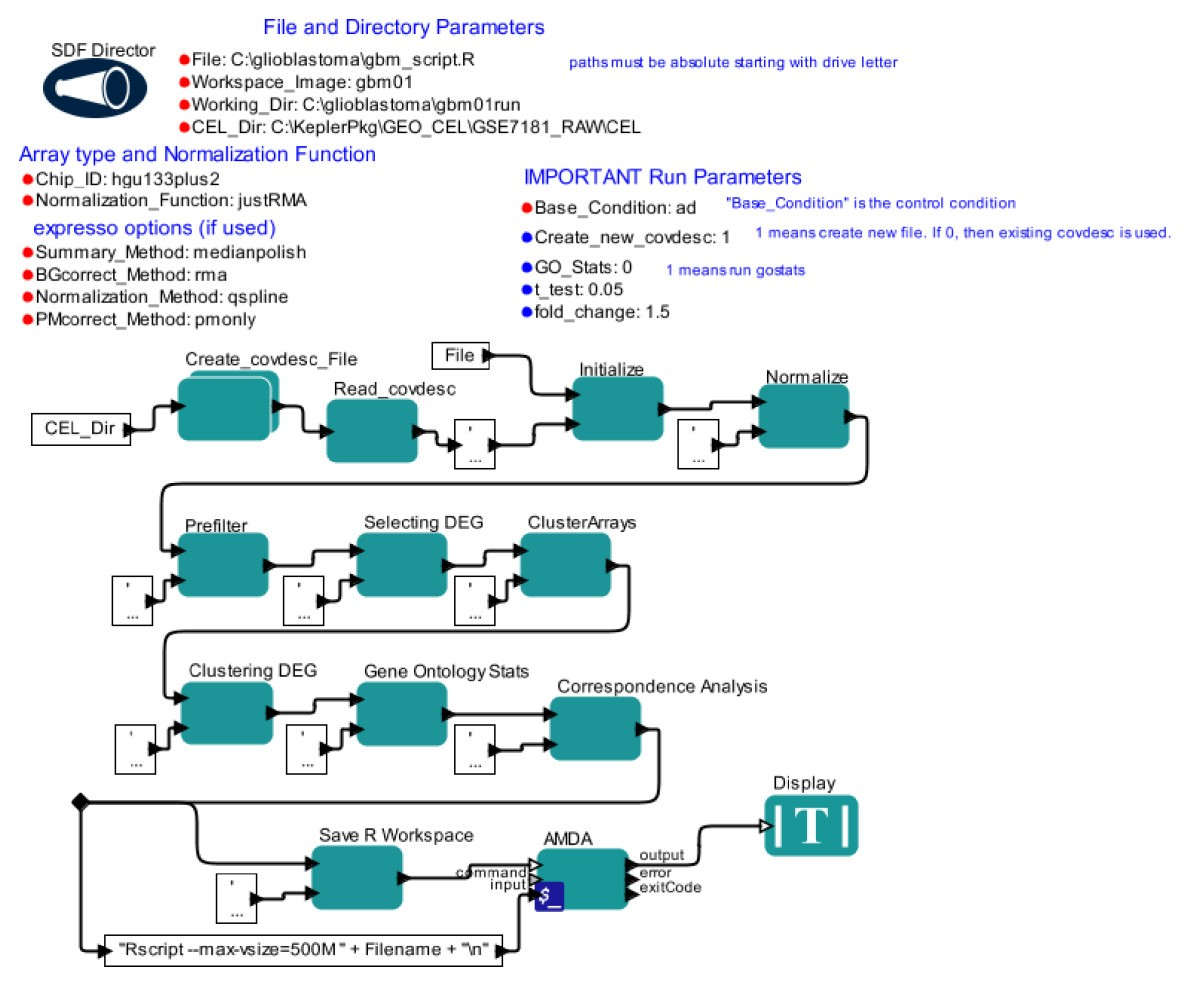
\includegraphics[height=0.35\textheight]{figures/screenshot.KeplerWorkflow.jpg}
  \caption{Описание процесса обработки данных в системе Kepler}
  \label{fig:intro.keplerScreenshot}
\end{figure}

Кроме того, для облегчения процесса разработки трудоёмкого ПО существуют т.н. платформы малокодовой разработки (англ.~low-code development platforms, \glsxtrshort{LCPD})\cite{DiRuscio2022}. В них, подобно системам управления потоком задач, логика разрабатываемого программного продукта описывается при помощи некоторого формального языка или с использованием графического редактора. От системы к системе подход к описаниям варьируется. Может применяться структурный подход, описывающий шаги алгоритма, или предметно-ориентированный, при котором описываются взаимодействующие сущности. Некоторые системы позволяют по созданному описанию генерировать готовые компоненты будущего программного продукта. Так платформа Codebots реализует предметно-ориентированный подход и по составленным UML-диаграммам взаимодействующих сущностей позволяет генерировать \glsxtrshort{API}, \glsxtrshort{JSON}-схемы данных и документацию\cite{DiRuscio2022}. Тем не менее, при реализации сложных вычислительных методов целесообразнее использовать структурный подход.

Одной из ключевых особенностей описанных технологических решений является выделение операций обработки данных в отдельные программные модули (функции, подпрограммы, скрипты). Как правило, при создании описаний алгоритмов в них используется следующий подход. Поскольку известно, что выходные данные одного программного модуля могут являться входными для одного или нескольких других модулей, можно сказать, что между ними формируются зависимости по входным и выходным данным. Тогда возможно составить такой ориентированный граф, описывающий общую логику алгоритма, в котором узлами являются операции обработки данных, а рёбрами -- пути данных. Такой подход получил название ``диаграммы потоков данных'' (англ.~Dataflow Diagram, \glsxtrshort{DFD}). На рисунке~\ref{fig:exampleDataflow} приведён пример такого ориентированного графа, описывающего процесс вычисления среднего арифметического и среднего геометрического двух массивов вещественных чисел.
\begin{figure}
  \centering
  \includegraphics[width=\textwidth]{figures/example.dataflow.png}
  \caption{Пример диаграммы потоков данных}
  \label{fig:exampleDataflow}
\end{figure}

При известных входных и выходных данных каждого модуля они могут создаваться независимо друг от друга\cite{DanilovPar2011}. Возникает возможность распределения задач создания отдельных программных модулей между разработчиками. Таким образом, уменьшается объём работы по написанию исходных кодов, приходящийся на одного исследователя. Это в свою очередь облегчает отладку и написание документации, что положительно сказывается на общем качестве реализуемого ПО.

В приведённом выше подходе существует необходимость явно описывать входные и выходные данные каждого процесса обработки. При этом на начальных этапах проектирования не всегда данные требуемые данные могут быть полность определены в силу недостатка представлений о программной реализации тех или иных этапов. Таким образом, в некоторых случаях может быть целесообразен такой подход к построению описания логики реализуемого решения, что в нём не указываются конкретные обрабатываемые данные. Последовательность выполнения отдельных этапов в таком случае должна задаваться явно. В предпринимательстве и управлении проектами подобный подход широко распространён и реализован в сетевых графиках. Сетевой график представляет собой ориентированный граф, в котором вершины -- это события или состояния проекта, а рёбра -- это работы. В работе~\cite{SokolovPershin2018} рассматривается применение идеи переходов между состояниями при описании логики вычислительных алгоритмов. Описанный подход получил название graph-based software engineering (\glsxtrshort{GBSE}). Кроме того в указанной работе описана реализация GBSE в библиотеке comsdk для языка C++.

Был проведён сравнительный анализ программного каркаса comsdk с аналогичным программным комплексом, в котором реализованы диаграммы потоков данных. В качестве такой реализации был рассмотрен программный комплекс pSeven, разработанный отечественной компанией DATADVANCE. Он направлен в первую очередь на решение конструкторских, оптимизационных задач и, помимо этого, задач анализа данных, что в первом приближении делает его аналогом comsdk по предметному назначению.

В терминах \textsf{pSeven}: графовое описание процесса решения задачи называется \textit{расчетной схемой} (англ.~workflow); вершинам графового описания поставлены в соответствие процессы обработки данных (используется термин \textit{блоки}), а рёбра определяют \textit{связи} между блоками и направления передачи данных между процессами~\cite{NazarenkoDFM2015}. При работе с pSeven используются следующие понятия:
\begin{itemize}
  \item \textsf{расчётная схема} -- формальное описание процесса решения некоторой задачи в виде ориентированного графа;
  \item \textsf{блок} -- программный контейнер для некоторого процесса обработки данных, входные и выходные данные для которого задаются через порты (см.~ниже);
  \item \textsf{порт} -- переменная конкретного\footnote{Динамическая типизация не поддерживается.} типа, определённая в блоке и имеющая уникальное имя в его пределах;
  \item \textsf{связь} -- направленное соединение типа ``один к одному'' между выходным и входным портами разных блоков.
\end{itemize}

С учётом данных понятий можно описать используемую методологию диаграмм потоков данных следующим образом. Расчётная схема содержит в себе набор процессов обработки данных (блоков), каждый из которых имеет (возможно, пустой) набор именованных входов и выходов (портов). Данные передаются через связи. Для избежания т.н. гонок данных (англ.~data races) множественные связи с одним и тем же входным портом не поддерживаются. Для начала выполнения каждому блоку требуются данные на всех входных портах. Все данные на выходных портах формируются по завершении исполнения блока~\cite{NazarenkoDFM2015}.

Сравнение реализаций двух подходов проводилось по следующим критериям:
\begin{itemize}
  \item особенности реализуемого подхода,
  \item особенности программной реализации,
  \item особенности взаимодействия пользователя с реализованной системой.
\end{itemize}
С учётом этого были выделены конкретные признаки для сравнения:
\begin{itemize}
  \item предметное назначение,
  \item значение вершины графа, описывающего алгоритм,
  \item значение ребра графа, описывающего алгоритм,
  \item топология графа, описывающего решение,
  \item поддержка иерархических графовых описаний, когда одно графовое описание является частью (ребром или вершиной) другого
  \item принцип передачи данных между отдельными этапами описываемого алгоритма,
  \item необходимость указывать входные и выходные данные каждого шага алгоритма
  \item язык программной реализации,
  \item файловый формат графовых описаний,
  \item файловая структура проекта реализуемого алгоритма,
  \item поддерживаемые типы данных,
  \item принцип ввода входных данных для алгоритма и его параметров,
  \item принцип вывода результатов работы алгоритма,
  \item поддержка параллельного выполнения незавимых шагов алгоритма,
  \item поддержка распределённого выполнения отдельных этапов алгоритма на вычислительном кластере,
  \item наличие графического редактора графовых описаний
  \item средства визуализации результатов работы алгоритма,
  \item поддержка алгоритмов, требующих принятие решения от пользователя,
  \item возможность дополнения набора входных данных во время работы алгоритма.
\end{itemize}

Результаты проведённого сравнения представлены в таблице \ref{rndhpcblo.0209}.

\begin{landscape}
  \begin{longtable}{|c|p{0.3\textwidth}|p{0.55\textwidth}|p{0.55\textwidth}|}
    \caption{Сравнительная таблица}\label{rndhpcblo.0209}                                                                                                                                                                                                                                                                                                                                                                                                                                                                                                                                                                                                                                                                                                                                                                                                                                                                                                                                                                                                           \\
    \hline
    \textbf{№} & \textbf{Признак}                                                                           & \textbf{pSeven}                                                                                                                                                                                                                                                                                                                                                                                                                                                                                                                                                                                                                                                   & \textbf{comsdk}                                                                                                                                                                                                                                                                   \\
    \hline
    1          & Предметное назначение                                                                      & Задачи оптимизации, анализ данных                                                                                                                                                                                                                                                                                                                                                                                                                                                                                                                                                                                                                                 & Задачи автоматизированного проектирования, алгоритмизация сложных вычислительных методов, анализ данных                                                                                                                                                                           \\
    \hline
    2          & Значение вершины графа, описывающего алгоритм                                              & Блок (процесс обработки данных)                                                                                                                                                                                                                                                                                                                                                                                                                                                                                                                                                                                                                                   & состояние данных                                                                                                                                                                                                                                                                  \\
    \hline
    3          & Значение ребра графа, описывающего алгоритм                                                & Связь (направление передачи данных)                                                                                                                                                                                                                                                                                                                                                                                                                                                                                                                                                                                                                               & переход меду состояниями с указанием функций, осуществляющих переход                                                                                                                                                                                                              \\
    \hline
    4          & Топология графа, описывающего решение                                                      & По умолчанию поддерживаются только ациклические графы. Поддерживаемая топология расширяется засчёт специальных управляющих блоков, которые отслеживают выполнение условий: для условного ветвления используется блок "Условие" (англ. condition), который перенаправляет данные на один из выходных портов в зависимости от выполнения описанного условия (подробнее см. \cite{pSevenDocsConditons2022}); Для реализации циклов в общем случае используются блоки "Цикл" (англ. loop)\cite{pSevenDocsWorkflow2021}, но для некоторых задач существуют специализированные блоки, организующие логику работы цикла (например, блок "Оптимизатор" (англ.~optimizer)) & Любая                                                                                                                                                                                                                                                                             \\
    \hline
    5          & Поддержка иерархических графовых описаний                                                  & \multicolumn{2}{c|}{Присутствует}                                                                                                                                                                                                                                                                                                                                                                                                                                                                                                                                                                                                                                                                                                                                                                                                                                                                                                                     \\
    \hline
    6          & Принцип передачи данных между отдельными этапами описываемого алгоритма                    & Данные между узлами передаются согласно определйнным связям, которые на уровне выполнения создают пространство в памяти для ввода и вывода данных для выполняемых в раздельных процессах блоков. Транзитная передача данных, которые не изменяются в данном блоке, на выход невозможна.                                                                                                                                                                                                                                                                                                                                                                           & Поскольку узлами графа являются состояния данных, существует возможность задействовать в расчётах только часть данных, оставляя их другую часть неизменной. Фактической передачи данных не производится.                                                                          \\
    \hline
    7          & Необходимость указывать входные и выходные данные каждого шага алгоритма                   & Присутствует                                                                                                                                                                                                                                                                                                                                                                                                                                                                                                                                                                                                                                                      & Отсутствует                                                                                                                                                                                                                                                                       \\
    \hline
    8          & Язык программной реализации                                                                & \multicolumn{2}{c|}{С++, Python}                                                                                                                                                                                                                                                                                                                                                                                                                                                                                                                                                                                                                                                                                                                                                                                                                                                                                                                      \\
    \hline
    9          & Файловый формат графовых описаний                                                          & Расчетная схема (в форме орграфа) сохраняется в двоичный файле закрытого формата с расширением \textsf{.p7wf}.                                                                                                                                                                                                                                                                                                                                                                                                                                                                                                                                                    & Графовая модель (определяет алгоритм проведения комплексных вычислений в форме орграфа) сохраняется в текстовом файле открытого формата, подготовленного на языке \gls{aDOT}\cite{SokolovADOT2020}, являющегося ``сужением'' (частным случаем) известного формата DOT (Graphviz). \\
    \hline
    10         & Файловая структура проекта реализуемого алгоритма                                          & Проект состоит из непосредственно файла проекта, в котором хранятся ссылки на созданные расчётные схемы и локальную базу данных, сами расчётные схемы, файлы с их входными данными, файлы отчётов, где сохраняются выходные данные последних расчётов и результаты их анализа.                                                                                                                                                                                                                                                                                                                                                                                    & Проект состоит из \textsf{.aDOT} файла с описанием графа, \textsf{.aINI}-файлов с описанием форматов входных данных, библиотек функций-обработчиков, функций-предикатов и функций-селекторов, файлов, куда записываются выходные данные.                                          \\
    \hline
    11         & Поддерживаемые типы данных                                                                 & Целые числа, числа с плавающей точкой, строки, логические переменные, логические, целочисленные и вещественные векторы и матрицы                                                                                                                                                                                                                                                                                                                                                                                                                                                                                                                                  & Целые и вещественные числа, строки, целочисленные и вещественные векторы                                                                                                                                                                                                          \\
    \hline
    12         & Принцип ввода входных данных для алгоритма и его параметров                                & Входные данные должны быть указаны при настройках внешних входных портов расчётной схемы.                                                                                                                                                                                                                                                                                                                                                                                                                                                                                                                                                                         & Входные данные хранятся в файле в формате \gls{aINI}\cite{SokAINI}, откуда считываются при запуске обхода графа~\cite{SokolovPershin2017}.                                                                                                                                        \\
    \hline
    13         & Принцип вывода результатов работы алгоритма                                                & Данные с выходных портов схемы сохраняются в локальной базе данных. Для их записи в файлы для обработки/анализа вне pSeven необходимо воспользоваться специально предназначенными для этого блоками.                                                                                                                                                                                                                                                                                                                                                                                                                                                              & Для записи выходных/промежуточных данных в файлы или базы данных необходимо добавить соответствующие функции-обработчики. Формат выходных данных не регламентирован.                                                                                                              \\
    \hline
    14         & Поддержка параллельного выполнения независимых шагов алгоритма                             & Присутствует. Блоки, входящие в состав различных ветвлений схемы могут быть выполнены параллельно, поскольку они не зависят друг от друга по используемым данным.                                                                                                                                                                                                                                                                                                                                                                                                                                                                                                 & Присутствует. Существует возможность обойти различные ветвления графа одновременно.                                                                                                                                                                                               \\
    \hline
    15         & Поддержка распределённого выполнения отдельных этапов алгоритма на вычислительном кластере & Присутствует                                                                                                                                                                                                                                                                                                                                                                                                                                                                                                                                                                                                                                                      & В текущей версии отсутствует                                                                                                                                                                                                                                                      \\
    \hline
    16         & Наличие графического редактора графовых описаний                                           & Да                                                                                                                                                                                                                                                                                                                                                                                                                                                                                                                                                                                                                                                                & Да\footnote{В виде отдельного веб-приложения}                                                                                                                                                                                                                                     \\
    \hline
    17         & Средства визуализации результатов работы алгоритма                                         & Реализованы как часть системы формирования отчётов (см. выше)                                                                                                                                                                                                                                                                                                                                                                                                                                                                                                                                                                                                     & В текущей версии отсутствуют                                                                                                                                                                                                                                                      \\
    \hline
    18         & Поддержка алгоритмов, требующих принятие решения от пользователя                           & По умолчанию отсутвует. Требуется реализация дополнительных скриптов на языке Python, отвечающих за взаимодействие с пользователем                                                                                                                                                                                                                                                                                                                                                                                                                                                                                                                                & Частично присутствует засчёт средства генерации форм ввода\cite{SokolovPershin2017}                                                                                                                                                                                               \\
    \hline
    19         & Возможность дополнения набора входных данных во время работы алгоритма                     & Отсутствует                                                                                                                                                                                                                                                                                                                                                                                                                                                                                                                                                                                                                                                       & Частично реализована при помощи функций-обработчиков специального типа, создающих формы ввода                                                                                                                                                                                     \\
    \hline
  \end{longtable}
\end{landscape}

Таким образом, на данный момент comsdk обладает сравнительно меньшим числом функциональных возможностей, чем современные научные системы управления потоком задач, подобные pSeven, но предоставляет потенциально больше средств для взаимодействия реализуемых алгоритмов с пользователем. В условиях существующей на сегодняшней день потребности в отечественном программном обеспечении для реализации сложных численных методов, актуально развитие данного программного каркаса.
%---------------------------------------------
\section{Постановка задачи}
%%%%%%%%%%%%%%%%%%%%%%%%%%%%%%%%%%%%%%%%%%%
\subsection{Концептуальная постановка задачи}
%%%%%%%%%%%%%%%%%%%%%%%%%%%%%%%%%%%%%%%%%%%
\begin{frame}%[allowframebreaks=0.9,t]

\begin{block}{Объект исследований}
\textexample{\ObjectOfResearch}
\end{block}

\begin{block}{Цель исследования}
\textexample{\GoalOfResearch}
\end{block}

\begin{block}{Задачи исследования}
\begin{enumerate}
	\arrowitem{Сравнить подходы к реализации графоориентированного подхода к решению задач проектирования на примере нескольких существующих программных комплексов}
	\arrowitem{Исследовать программную структуру модуля каркаса GBSE, отвечающего за струкутуру графовых моделей}
	\arrowitem{Определить требования к структуре данного модуля}
	\arrowitem{Разработать новую структуру, которая бы отвечала сформулированным требованиям}
\end{enumerate}
\end{block}

\end{frame}

%%%%%%%%%%%%%%%%%%%%%%%%%%%%%%%%%%%%%%%%%%%
\subsection{Требования к программной реализации структуры данных <<графовая модель>>}
%%%%%%%%%%%%%%%%%%%%%%%%%%%%%%%%%%%%%%%%%%%
\begin{frame}%[allowframebreaks=0.9,t]

\begin{itemize}
	\item Должна обеспечиваться поддержка актуальной версии формата aDOT~\footcite{SokADOT}.
	\item Реализуемая структура данных должна содержать в себе все узлы и рёбра, относящиеся к данной графовой модели.
	\item Топология графовой модели должна описываться матрицей смежности.
	\item Реализуемая структура данных должна предоставлять интерфейс для доступа к данным о топологии.
\end{itemize}

\end{frame}

%%%%%%%%%%%%%%%%%%%%%%%%%%%%%%%%%%%%%%%%%%%
\subsection{Требования к программной реализации структуры данных узла графовой модели}
%%%%%%%%%%%%%%%%%%%%%%%%%%%%%%%%%%%%%%%%%%%
\begin{frame}[t]
	\begin{itemize}
		\arrowitem{Реализуемая струкутра данных должна содержать в себе:}
		\begin{itemize}
			\item описание состояния данных (в некотором внутреннем формате);
			\item стратегию параллельного исполнения\footnote{т.е. данные о том, как параллельно исполнять исходящие из данного узла рёбра};
			\item функцию-селектор (или ссылку на неё).
		\end{itemize}
		\arrowitem{Реализуемая структура данных должна предоставлять интерфейс для:}
		\begin{itemize}
			\item назначения стратегию параллельного выполнения;
			\item назначения функции-селектора;
			\item вызова функции селектора с заданным набором данных.
		\end{itemize}
	\end{itemize}
	\begin{figure}
		\includegraphics[height=0.4\textheight]{images/graph.node_data.png}
	\end{figure}
\end{frame}

%%%%%%%%%%%%%%%%%%%%%%%%%%%%%%%%%%%%%%%%%%%
\subsection{Требования к программной реализации структуры данных ребра графовой модели}
%%%%%%%%%%%%%%%%%%%%%%%%%%%%%%%%%%%%%%%%%%%
\begin{frame}%[allowframebreaks=0.9,t
	\begin{itemize}
		\arrowitem{Реализуемая структура должна содержать в себе до трёх структур данных (или ссылок на них) типа <<морфизм>> -- препроцессор, обработчик и постпроцессор.}
		\arrowitem{Функциональная структура данных типа <<морфизм>> должна содержать в себе:}
		\begin{itemize}
			\item ссылку на функцию-предикат;
			\item ссылку на функцию-обработчик;
		\end{itemize}
		\arrowitem{Реализуемая структура должна предоставлять интефейс для:}
		\begin{itemize}
			\item назначения препроцессора, обработчика и постпроцессора;
			\item вызова хранящихся в ней <<морфизмов>> с заданным входным набором данных.
		\end{itemize}
	\end{itemize}
	\begin{figure}
		\includegraphics[height=0.275\textheight]{images/graph.edge_data.png}
	\end{figure}
\end{frame}


%---------------------------------------------
\section{Архитектура программной реализации}
%%%%%%%%%%%%%%%%%%%%%%%%%%%%%%%%%%%%%%%%%%%%%%%%%%%%%%%%%%%%%%%%
\subsection{Текущая реализация описанного подхода}
%%%%%%%%%%%%%%%%%%%%%%%%%%%%%%%%%%%%%%%%%%%%%%%%%%%%%%%%%%%%%%%%
\begin{frame}
	В библиотеке comsdk, являющейся реализацией описанного выше подхода на языке C++, помимо прочих описаны следующие структуры данных:
	\begin{itemize}
		\item \textsf{Anymap} -- ассоциативный массив, позволяющий хранить в себе разнотипные данные;
		\item \textsf{ActionItem} -- функциональный объект, реализующий функцию-обработчик;
		\item \textsf{ActionItemContext} -- объект, осуществляющий запуск функций-обработчиков и хранящий данные об их выполнении;
		\item \textsf{Predicate} -- функциональный объект, являющийся обёрткой над некоторой функцией, ставящей в соответствие входному набору данных логическое значение (0 или 1);
	\end{itemize}	
\end{frame}

%%%%%%%%%%%%%%%%%%%%%%%%%%%%%%%%%%%%%%%%%%%%%%%%%%%%%%%%%%%%%%%%
\subsection{Предлагаемая структура данных узла графовой модели}
%%%%%%%%%%%%%%%%%%%%%%%%%%%%%%%%%%%%%%%%%%%%%%%%%%%%%%%%%%%%%%%%
\begin{frame}%[allowframebreaks=0.9,t]
	Структуры данных разрабатывались с учётом возможностей стандарта C++-11 и библиотеки Standart Template Library (STL). Для описания разработанных структур данных был использован язык графического описания UML (Unified Modeling Language).
	\begin{figure}
		\begin{minipage}{0.49\textwidth}
			\centering
			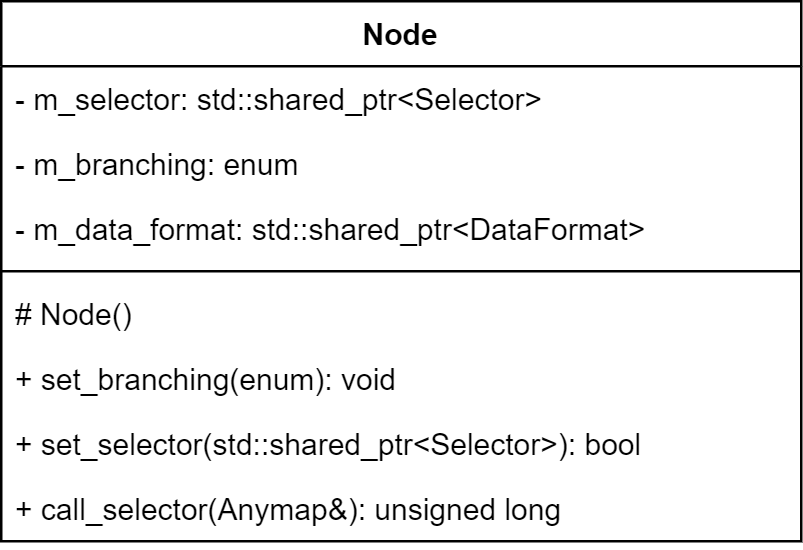
\includegraphics[width=\textwidth]{images/class.node.png}
			\caption{UML-диаграмма класса узла графа}
		\end{minipage}\hfill\begin{minipage}{0.49\textwidth}
			\begin{itemize}
				\item Использует умные указатели (\textsf{shared_ptr}) -- эффективное использование памяти.
				\item Защищённый конструктор -- объекты данного класса создаются только в пределах класса графовой модели.
				\item Интерфейс и информационные поля соответствуют требованиям.
			\end{itemize}
		\end{minipage}
	\end{figure}
\end{frame}
%%%%%%%%%%%%%%%%%%%%%%%%%%%%%%%%%%%%%%%%%%%%%%%%%%%%%%%%%%%%%%%%
\subsection{Предлагаемая структура данных ребра графовой модели}
%%%%%%%%%%%%%%%%%%%%%%%%%%%%%%%%%%%%%%%%%%%%%%%%%%%%%%%%%%%%%%%%
\begin{frame}%[allowframebreaks=0.9,t]
	\begin{figure}
		\begin{minipage}{0.49\textwidth}
			\begin{itemize}
				\item Использует умные указатели (\textsf{shared_ptr}) -- эффективное использование памяти.
				\item Защищённый конструктор -- объекты данного класса создаются только в пределах класса графовой модели.
				\item Интерфейс и информационные поля соответствуют требованиям.
				\item Для прохода по ребру необходимо назначить ему хотя бы одну пару предикат-обработчик (объединённых в структуру данных \textsf{Morphism}) с помощью метода set_function.
			\end{itemize}
		\end{minipage}\hfill\begin{minipage}{0.49\textwidth}
			\centering
			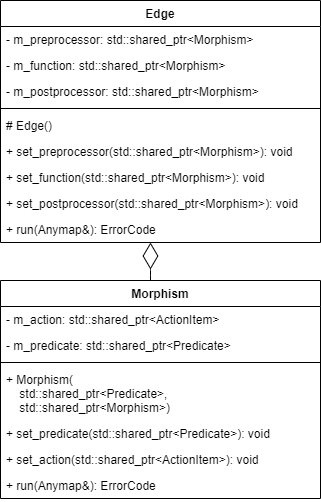
\includegraphics[height=0.75\textheight]{images/class.edge.png}
			\caption{UML-диаграмма класса ребра графа}
		\end{minipage}
	\end{figure}
\end{frame}

%%%%%%%%%%%%%%%%%%%%%%%%%%%%%%%%%%%%%%%%%%%%%%%%%%%%%%%%%%%%%%%%
\subsection{Предлагаемая структура данных графовой модели}
%%%%%%%%%%%%%%%%%%%%%%%%%%%%%%%%%%%%%%%%%%%%%%%%%%%%%%%%%%%%%%%%
\begin{frame}%[allowframebreaks=0.9,t]
	\begin{figure}
		\begin{minipage}{0.49\textwidth}
			\centering
			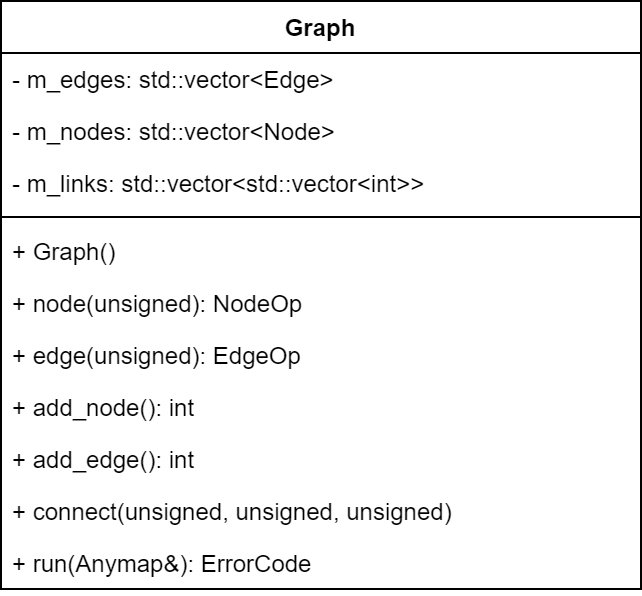
\includegraphics[width=0.8\textwidth]{images/class.graph.png}
			\caption{UML-диаграмма класса графа}
		\end{minipage}\hfill\begin{minipage}{0.49\textwidth}
			\begin{itemize}
				\item Хранит в себе узлы и рёбра графовой модели.
				\item Хранит в себе динамическую матрицу смежности.
				\item Позволяет добавлять узлы и рёбра и связывать их.
				\item Позволяет запустить обход графовой модели с заданным набором входных данных.
			\end{itemize}
		\end{minipage}
	\end{figure}
\end{frame}
%%%%%%%%%%%%%%%%%%%%%%%%%%%%%%%%%%%%%%%%%%%%%%%%%%%%%%%%%%%%%%%%
\subsection{Дополнительные структуры данных}
%%%%%%%%%%%%%%%%%%%%%%%%%%%%%%%%%%%%%%%%%%%%%%%%%%%%%%%%%%%%%%%%
\begin{frame}
	\begin{figure}
		\begin{minipage}{0.49\textwidth}
			\begin{itemize}
				\item NodeOp -- сокращение от ``Node Operation''.
				\item Дополнительная структура данных для операций с узлами.
				\item Хранит только индекс узла -- эффективное использование памяти.
				\item Позволяет получить соседние узлы для данного узла;
				\item Позволяет получить входящие и исходящие рёбра для данного узла;
				\item Позволяет при необходимости обратиться к интерфейсу самого узла.
			\end{itemize}
		\end{minipage}\hfill\begin{minipage}{0.49\textwidth}
			\centering
			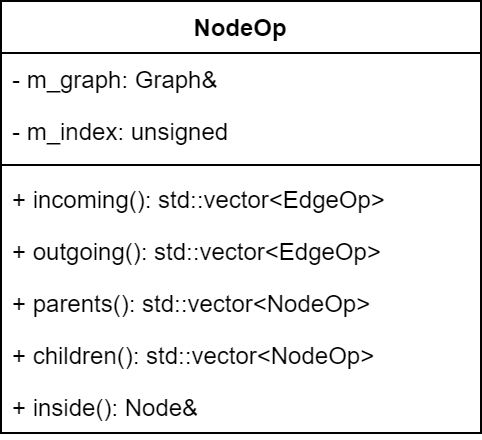
\includegraphics[width=0.75\textwidth]{images/class.nodeop.png}
			\caption{UML-диаграмма класса операции с узлом}
		\end{minipage}
	\end{figure}
\end{frame}

\begin{frame}
	\begin{figure}
		\begin{minipage}{0.49\textwidth}
			\begin{itemize}
				\item EdgeOp -- сокращение от ``Edge Operation''
				\item Дополнительная структура данных для операций с рёбрами.
				\item Хранит только индекс ребра -- эффективное использование памяти.
				\item Позволяет получить начальный и конечный узлы для данного ребра.
				\item Позволяет при необходимости обратиться к интерфейсу самого ребра.
			\end{itemize}
		\end{minipage}\hfill\begin{minipage}{0.49\textwidth}
			\centering
			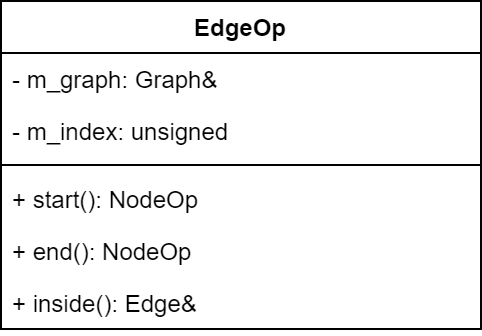
\includegraphics[width=0.75\textwidth]{images/class.edgeop.png}
			\caption{UML-диаграмма класса операции с ребром}
		\end{minipage}
	\end{figure}
\end{frame}
%%%%%%%%%%%%%%%%%%%%%%%%%%%%%%%%%%%%%%%%%%%%%%%%%%%%%%%%%%%%%%%%

%---------------------------------------------
\section*{Заключение}
%----------------------------------------------------------
\chapter*{ЗАКЛЮЧЕНИЕ}\label{chap_conclusion}
\addcontentsline{toc}{chapter}{ЗАКЛЮЧЕНИЕ}
%----------------------------------------------------------

В результате проведенной работы был реализован редактор графов, который является достаточно полезным инструментом, дополняющим предложенный А.П.Соколовым и А.Ю.Першиными графоориетированный программный каркас для реализации сложных вычислительных методов. Редактор позволяет создавать ориентированный граф с нуля, а затем экспортировать созданный граф в формате aDOT, также есть возможность загрузить граф из формата aDOT. С помощью редактора можно получить графовую модель вычислительно метода до его реализации, что позволяет заранее распределить задачи между разработчиками, а также, возможно, увидеть тонкие места в реализуемом методе и уделить им особое внимание. 

%----------------------------------------------------------

%---------------------------------------------
\def\secname{}

\begin{frame}

\begin{center}
\LARGE
Спасибо за внимание!
\vspace{1cm}

Вопросы?
\end{center}

\end{frame}
%---------------------------------------------
\section*{Приложение. Основная терминология}
%---------------------------------------------
\begin{frame}[allowframebreaks=0.9,t]

\printglossary[style=index, type=\acronymtype, title=Аббревиатуры, nopostdot=false]
%\printglossary[style=index, type=main, title=Термины и определения, nopostdot=true]

\end{frame}
%---------------------------------------------
\end{document}
%---------------------------------------------



